

\chapter{Testing} \label{chap:test}
With types of behavior now being detected, the next step is to validate that the scripts function correctly and without impacting the execution to heavily. This section will describe the different testing methods we employed to make sure the system behaved correctly.

\section{Testing the Event Engine modifications}
The first step towards validating the system was verifying that the new events themselves worked as intended. In order to do this, we created a small auxiliary script which would have a very basic functionality: every time an MPTCP event is seen, it prints out the event type and all the values contained in the event to the standard output. Next, we created a short packet capture in which we visited an MPTCP-enabled website: \url {https://amiusingmptcp.com/} \cite{amiusing}. We checked the capture with Wireshark \citep{wireshark} which quickly showed us that the capture contained enough MPTCP behavior to run some tests. The capture contains two MPTCP connection establishments, each one of which advertise several other addresses on which new subflows are created, using both IPv4 and IPv6. \\

We then ran Bro on our new capture, specifying that our script should be loaded. the result was as expected, with the contents of the MPTCP options being printed out to the console. In order to verify that the content was correct, we performed a side-by-side comparison of the values that Bro output, and those visible via Wireshark.

\section{Testing the Logging}
In section \ref{section:mp log}, we describe how we wrote a script which would log all the TCP connections that used MPTCP while matching subflows to their respective MPTCP connection. This script was tested in two phases. First, we ran it over the same capture we used to test the events. The number of packets and connections was small enough that we could use Wireshark to compare the output log to what we saw hands-on. By following the capture packet by packet, we saw which connections were established with MP Capable, making them initial subflows for their MPTCP connections. The first TCP flow that was established with a MP Join happened before the second MPTCP connection was established, allowing us to easily view the token corresponding to the first connection. From then on, we could count the flows by hand and make sure each one was attributed to the correct MPTCP connection in the log. \\

We also used this occasion to make sure the data structures we were using were being emptied out as the analysis progressed by periodically printing out the content of the tables. \\

Once we had ascertained that the log satisfied our requirements, we ran the script both on a large packet capture containing visits and downloads from multiple TCP-enabled websites, and on a live Ethernet interface while browsing the web. In both cases, we were not expecting to be able to validate that the contents of the log exactly matched what had happened. The test was mainly to make sure no odd behavior, errors, or incorrect log entries appeared.

\section{Testing the Bad Behavior Detection}
The last remaining script functions to test were those making use of the notice framework for the detecting and notification or odd behavior. These tests also took place in two phases. First, we ran them over a series of large packet captures, and a live Ethernet capture. The main focus of this test was to make sure the script was not raising any false positives. Real MPTCP traffic is not expected to trigger any of our notices, and therefore nothing should be printed out. There is one exception though: the \texttt{Duplicate\_add\_addr}. As we saw in section \ref{section:add addr log}, this notice is raised in two different cases, with a different message depending on the situation. The truly bad case is the advertisement of a new address on an existing address ID, but we also raised a notice when the same address and port pair was advertised on the same address ID. This is a case that is allowed, but where the receiver should normally ignore the duplicate advertisement. This second type of \texttt{Duplicate\_add\_addr} did appear during the first test, but none of the other notices were raised. \\

The second phase of the testing was to make sure the notices would be raised should the situation ever call for it.  In order to test this, we would need packet captures showcasing behavior that only a bad implementation of MPTCP would generate. Since such captures are not readily available, we turned to the packet manipulation program Scapy \citep{scapy}, and more particularly the MPTCP adaption of the software \citep{mpscapy}. Thanks to this program we were able to write short packets captures which contained the specific behavior we were attempting to detect. Due to certain limitations of the program (packets containing certain types of options such as IPv6 ADD ADDR could not be written to pcap files), we limited ourselves to just the behavior we needed, resulting in very short traces containing only a few signaling packets.\\

For the detection of duplicate address IDs, we started by taking the short trace we used for earlier testing. As mentioned before, this trace contains, along other things, the establishment of an MPTCP connection, the advertisement of several addresses, and the establishment of other subflows that join the connection. We then copied the three packets of the connection establishment, as well as the first address advertisement into a new packet list. Then, we copied the address advertisement into another packet. It advertised an IPv4 address, needed since the program could not print out IPv6 Add Addr options, on the address ID 2. We modified the copy of the packet so that the address would be different. We then let Scapy recompute the TCP checksum and wrote the packet list to a new pcap. The result was a 5 packet capture in which we establish an MPTCP connection, then advertise two different IPv4 addresses on the same address ID. When the script was run against this capture, a notice was raised and printed out the correct ID and addresses. Figure \ref{pic:bad add} illustrates the content of the test trace.\\

\begin{figure}[!t]
\centering
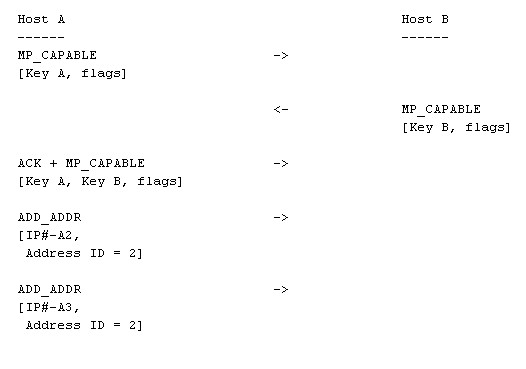
\includegraphics[scale = 0.75]{Figures/addpcap.png}
\caption{Generated Packet Capture for Duplicate Add Addr}
\label{pic:bad add}
\end{figure}

To verify whether our key change detection was working, we once again took our short trace. This trace was easier to create, we simply copied the SYN and SYN+ACK of the first connection establishment into a new packet list. Next, modified the two keys of the ACK packet and added our modified ACK to the packet list. We then wrote the three packets to a new capture. As in the previous case, the corresponding notice was raised when we ran the script on our generated trace, printing out both the old and new keys. The contents of our modified trace basically correspond to the interactions between Host A and the Server from figure \ref{pic:2 cap attack}. \\

Next, we move on the the Join flooding detection. In this case, we actually need a large trace in order to simulate a flood attack. Using Scapy and our trusty capture once more, we begin by copying one of the existing SYN packets with an MP Join option. Then, enter a loop in which we create a copy of this packet, change the sender address to a random one, recalculate the checksum, and append the copy into a new packet list. We did this 10.000 times, giving a trace with a large number of SYN packets by most standards. The threshold for detecting a Join flood was arbitrarily set at 1000 SYN's over 10 seconds. When we ran our script over the fabricated trace, the entire execution lasted less than the time interval, meaning we got 10.000 connection attempts within a single period. The notice was raised after the first 1000, as expected, and it was only raised once thanks to our suppression of the notice.

\section{Performance Testing}
The last step for the evaluation of our implementation is performance testing. For reproducible test, we limited the study to packet captures. Given that the engine is not limited by the speed at which the network delivers packets in this case, the execution time is not really representative of a real deployment. Therefore we focused on peak memory usage. Evidently, we want to compare the memory usage of Bro with and without our scripts to see of the generation and handling of event negatively impacts the system's performance.\\

We ran two test cases: in the first, Bro is executed on the Join flood packet capture, containing only 10.000 SYN packets. In the second case, we run Bro on a large packet capture with over 400k packets of regular network traffic. For both cases, we ran Bro 20 times while measuring the memory usage with a bash script \cite{memusg}. Table \ref{table:perf} summarizes the results of this test.\\

\begin{table}
\centering
\begin{tabular}{| c | c | c | c |}
\hline
 & No Script & With Script & Diff \\ \hline
Flood pcap & 142.207 & 142.117 & -0,06\% \\
(10k packets) & & & \\ \hline
Large pcap & 90.925 & 91.982 & +1,16\% \\
(400k+ packets) & &  & \\ \hline
\end{tabular}
\caption{Average Peak memory [KB] usage over 20 iterations}
\label{table:perf}
\end{table}

The first thing we can observe is that the difference between using the script and not using it is extremely small, and the MPTCP detection is therefore unlikely to cause more performance issues than a standard usage of Bro. This is likely due to the fact that that small amount of additional memory we are using in script pales before the large amount of state maintained by the Event Engine regardless of which events must be generated. \\

The second observation we can make is that, both with and without the script, the flood pcap cause a much higher peak memory usage despite but much smaller than the other capture. Once again, this points to the fact that the Event Engine is the main memory user. Regardless of whether we are looking for a flood attack, the Engine will create state for the connection attempts.